%================================================================
\section{Background}\label{sec:Theory}
%================================================================

\subsubsection*{New outline}

\begin{itemize}
    \item Just focus on dim reduction (no parameter estimation)
    \item Experiments
    \begin{itemize}
        \item Conv-VAE MNIST (f.ex. 0-4) *
        \item $\beta$-VAE MNIST *
        \item InfoVAE MNIST *
        \item InfoVAE HH *
        \item Maybe: InfoVAE OU *
        \item LSTM or Transformer VAE HH (deterministic)
        \item Maybe: try models on Ornstein–Uhlenbeck (OU) process (stochastic) \url{https://stat.pitt.edu/si/ou.pdf}
    \end{itemize}
    \item Model goodness qualitatively by comparing simulation vs generative model
    \item use t-SNE for visualizing latent space
    \item Quantitative:
    \begin{itemize}
        \item Reconstruction error over latent dimensionality
    \end{itemize}
\end{itemize}

\subsubsection*{Old outline}

\begin{itemize}
    \item Autoencoders (brief)
    \begin{itemize}
        \item Purpose
        \item Architecture
        \item Optimization (reconstruction loss)
    \end{itemize}
    \item Variational autoencoders
    \begin{itemize}
        \item Key difference between AE and VAE
        \item VAE optimization (reconstruction loss + regularization)
        \item Reparametrization trick
    \end{itemize}
    \item $\beta$-VAE
    \item Convolutional VAE (maybe Method)
    \begin{itemize}
        \item Traditional CNN
        \item If time, modern CNN with Fourier transforms
    \end{itemize}
    \item LSTM-based VAE (maybe Method)
    \begin{itemize}
        \item RNN background
        \item LSTM
    \end{itemize}
    \item Latent perturbation / interpreting latent features 
\end{itemize}

%----------------------------------------------------------------
\subsection{Autoencoders}
%----------------------------------------------------------------

An autoencoder is a type of artificial neural network that employs dimensionality reduction techniques for data compression and feature extraction of a dataset. The aim of an autoencoder is to find a latent feature representation of the data. It consists of two main components: an encoder and a decoder. As depicted in \autoref{fig:ae}, the encoder processes an input, such as an image, and compresses it into a compact representation of latent features. This representation is the most reduced form of feature representation that still allows reconstruction of the original input within a defined quality threshold. Subsequently, the decoder reconstructs the input from the compressed representation. The training objective of an autoencoder is to minimize the reconstruction error compared to the original input. The choice of encoder/decoder is adapted to the type of input data. For instance, convolutional neural networks (CNNs) are typically used for image data, whereas recurrent neural networks (RNNs) are suited for sequential data, such as time-series data. 

\begin{figure}[!htb]
 \centering
 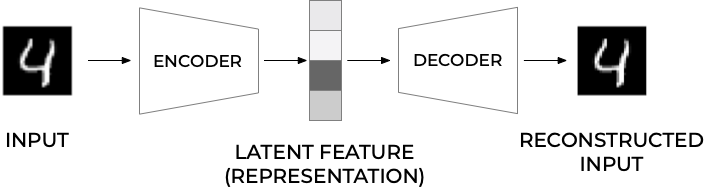
\includegraphics[scale=0.5]{ae1.png}
 % ae1.png: 711x193 px, 72dpi, 25.08x6.81 cm, bb=0 0 711 193
 \caption{\textbf{Autoencoder representation}: Here, an image depicting the digit 4 from the MNIST dataset is first sent through an encoder which compresses the image to a lower-dimensional (latent feature) representation. Then, the compressed representation is sent through a decoder which tries to reconstruct the original image.}
 \label{fig:ae}
\end{figure}

Although autoencoders are effective in data compression and reconstruction, there is no stochasticity involved. This makes them inadequate for generating new data that fits a specific class. For example, an autoencoder trained on images of chairs can recreate these specific chairs, but will not create a variety of new chair images encompassing the full concept of "chairness". Moreover, the latent space of regular autoencoders may be discontinuous, making the generation and interpretation of specific features challenging or impossible. To introduce stochasticity and create continuous and practical latent spaces, Variational Autoencoders (VAEs) can be used. VAEs improve upon standard autoencoders by incorporating probabilistic elements, allowing the generation of new data instances that conform to the desired class. 

\subsection{Variational Autoencoders}

In a simplified way, stochasticity in VAEs is introduced within the latent feature space (see \autoref{fig:ae}). Instead of storing a single output value per feature, VAEs store a probability distribution, represented by a mean and a standard deviation for each feature. This approach ensures that specific features are continuous around their mean (via the standard deviation) and sufficiently separated to be distinguishable (via the mean).

The probability distribution in the latent feature space allows for sampling, enabling the generation of new outputs that are both novel and recognizable as belonging to the intended class, despite not being present in the training data.

To develop an effective generative model, the aim is to maximize the marginal likelihood $p(x)$ over all $x$. This can be challenging, as it requires either knowing the true data distribution or performing an infeasible integral over latent parameters. The solution to this problem is to derive the Evidence Lower Bound (ELBO) where evidence is the log-likelihood of the input data. Given a parametrized encoder with the goal of being as close as possible to the ground truth distributions; $q_\phi(z|x)\approx p(z|x)$, ELBO can be represented by the following equation:

\begin{equation}\label{eqn:elbo}
 \mathbb{E}_{q_\phi(z|x)}\left[\log \frac{p(x,z)}{q_\phi(z|x)}  \right]
\end{equation}

%As the name tells us, this is the lower boundary, so in other words we wish to maximize this expression to optimize our model. By using the chain rule of probability on the expression for ELBO we can rewrite it as

Here, $q_\phi(z|x)$ is a parametrized encoder that approximates the true posterior distribution $p(z|x)$. The objective is to maximize the ELBO to optimize the model. By applying the chain rule of probability to this expression, the ELBO can be rewritten as:

\begin{equation}\label{eqn:loss}
 \mathbb{E}_{q_\phi(z|x)}\left[\log \frac{p(x,z)}{q_\phi(z|x)}  \right]
 = \mathbb{E}_{q_\phi(z|x)}[\log p_\theta (x|z)] -D_{KL}(q_\phi(z|x)||p(z))
\end{equation}

In this equation, $p_\theta(x|z)$ is a parametrized function that takes samples from the latent space $z$ to generate new output. Stochasticity is included in creating the latent space, making the function deterministic. The first term on the right-hand side represents the reconstruction error, ensuring that the latent features can recreate the input data. The second term is the Kullback-Leibler divergence, which measures the difference between two probability distributions.

It is important to note that the function $q_\phi(z|x)$ serves as an encoder, taking data from $x$ into $z$, while the function $p_\theta(x|z)$ serves as the decoder, transforming latent variable $z$ into output $x$. The first term on the right-hand side in \autoref{eqn:loss} can be interpreted as the reconstruction error. This term ensures the model's ability to generate accurate latent features that can be used to recreate input data. The second term is a regularization term that measures how similar the encoder's inferred latent distribution is to the prior $p(z)$. 

\subsubsection{$\beta$-VAE}

A challenge of VAE is that features in the latent space can become entangled. For exmple, in a VAE trained to generate faces, the feature controlling the head's angle might become entangled with the feature controlling the person's smile. Consequently, a generated person looking to the left might always appear sad, while one looking to the right might always appear happy. This issue can be resolved by introducing a hyperparameter $\beta >1$ in front of the KL-divergence term in the ELBO equation:

\begin{equation}\label{eqn:beta}
 \mathbb{E}_{q_\phi(z|x)}\left[\log \frac{p(x,z)}{q_\phi(z|x)}  \right]
 = \mathbb{E}_{q_\phi(z|x)}[\log p_\theta (x|z)] -\beta D_{KL}(q_\phi(z|x)||p(z))
\end{equation}


The $\beta$ parameter forces the model to consider the chosen prior distribution during optimization. For example, if a multivariate Gaussian is chosen as the prior, the model will force the encoded values closer to this distribution. By increasing the cost of adding features to the latent layer, $\beta$ reduces feature redundancy. In a VAE for generating faces, this means it would help eliminate unnecessary features, such as an extra feature encoding both hair and eye color when separate features for hair color and eye color already exist.

\subsubsection{InfoVAE}

Another potential challenge with VAEs is that the encoder can assign identical latent features to any input $x$. Consequently, when the decoder samples from this distribution, it effectively samples from the distribution of the input data rather than from meaningful and learned features. This issue may not be critical if the objective is solely to generate images with a VAE. However, if the goal is to utilize the encoder for specific tasks, such as identifying which measurable quantities are essential for generating particular experimental data, it becomes crucial to ensure that the latent space contains useful features.

InfoVAE addresses both this issue and the issue solved by $\beta$-VAE, as $\beta$-VAE is a special case of InfoVAE. To formulate the training objective of InfoVAE, it is instructive to start from an alternative, but equivalently constant, formulation of \autoref{eqn:loss} \citep{Zhao}

\begin{equation} \label{eqn:4}
 \mathbb{E}_{q_\phi(z|x)}\left[\log \frac{p(x,z)}{q_\phi(z|x)}  \right]
 =-D_{KL}(q_\phi(z)||p(z))-\mathbb{E}_{q_\phi(z)}[D_{KL}(q_\phi(x|z)||p_\theta(x|z))].
\end{equation}

Another issue in VAEs arises from the fact that the dimensionality of input $x$ is typically much larger than that of the feature space $z$. This is known as Modeling Bias and applies to both divergences in \autoref{eqn:4}. If these divergences increase inversely, the error from the last term on the right-hand side of \autoref{eqn:4} can dominate, rendering the divergences in the latent space insignificant.

To address all these issues inherent in standard VAEs, we modify the training objective in specific ways. To emphasize the importance of divergence in the latent space, we introduce a scaling hyperparameter $\lambda$ to multiply the first term on the right-hand side of \autoref{eqn:4}. Furthermore, we introduce a new term to counteract the tendency to underutilize samples $z$ from the latent space during decoding. This term is based on the mutual information between $z$ and $x$, denoted as $I_{q_\phi}(x,z)$. Since this term is positive, minimizing mutual information is desired. The revised objective for InfoVAE is then:

\begin{align}
 \mathbb{E}_{q_\phi(z|x)}\left[\log \frac{p(x,z)}{q_\phi(z|x)}  \right]_{InfoVAE}
 =&-\lambda D_{KL}(q_\phi(z)||p(z))\\ \nonumber
 &-\mathbb{E}_{q_\phi(z)}[D_{KL}(q_\phi(x|z)||p_\theta(x|z))]\\ \nonumber
 &+\alpha I_{q_\phi(x,z)}(x;z).
 \label{eqn:4}
\end{align}

where this formulation is not immediately straightforward to optimize. Returning to the standard ELBO is achieved by setting the hyperparameters to $\alpha=0$ and $\lambda=1$, while $\lambda > 0$ and $\alpha+\lambda-1=0$ return to $\beta$-VAE.

\subsection{MLP and DNN}

A multilayer perceptron (MLP) represents one of the fundamental types of neural networks, illustrated in Figure \ref{fig:mlp}. The network takes a set of inputs $X$, which are the features or data to be studied, and connects them to the subsequent hidden layer to the right through a series of weights, each corresponding to a connection. Each node $a$ in this hidden layer computes a weighted sum of inputs, augmented by a layer-specific bias term, and applies a non-linear activation function such as sigmoid, tanh, or ReLU. These activation functions introduce non-linearity into the model, enabling it to capture complex relationships between input variables and providing depth to the network (where multiple linear transformations cannot simply be replaced by a single linear transformation). The bias term adjusts the activation threshold of each node, analogous to a firing threshold in neuron models. The final layer $f(X)$ in \ref{fig:mlp} integrates outputs from the preceding layer to produce the network's final output value(s). To construct a more sophisticated and potentially more powerful network, additional hidden layers are often added successively. 


\begin{figure}[H]
    \centering
    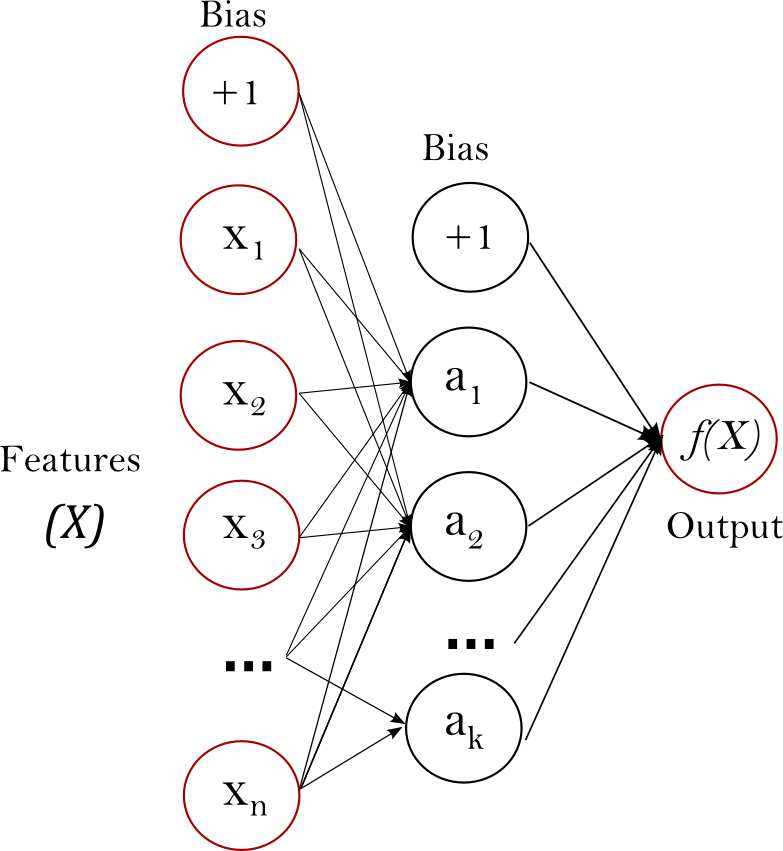
\includegraphics[width=0.5\linewidth]{latex//figures/multilayerperceptron_network.png}
    \caption{\textbf{MLP}:Input data $X$ is sent to a hidden layer, denoted $a$, and finally an output $f(X)$ is generated. Figure borrowed without permission from sckikit-learn.org.}
    \label{fig:mlp}
\end{figure}

Initially, the network will produce meaningless output until it is trained. Training involves adjusting the weights and biases for each hidden layer by comparing the generated output to known target data. For instance, when classifying digits from the MNIST dataset, a flattened array of grayscale values is input, and the network aims to classify them into digits 0 through 9. The error between the network's output and the correct answers is computed and propagated backward through the layers via backpropagation. At each layer, weights and biases are updated in accordance with the error to refine the model's predictions. Training continues iteratively until predefined criteria are met, such as reaching a specified number of iterations or no longer improving over several cycles. This process, known as model training, demands substantial amounts of data and computation time. A well-trained model with low error can then be deployed on unseen data to predict outputs that closely match the correct results.

A deep neural network (DNN) is constructed using the same fundamental elements as the MLP in \ref{fig:mlp}, but with increased complexity including additional hidden layers as illustrated in \ref{fig:dnn}. For instance, taking the input of 28x28 dimensions of MNIST data flattened to a 784-dimensional vector into consideration, MLP and DNN show different network architectures. In the case of MLP, the input is fed into a single hidden layer comprising 500 features, where the output, serving as the latent space in a VAE, is set to 20 features. DNN follows the same initial structures, but includes additional hidden layers subsequent to the first and features 150 features. Therefore, MLPs and DNNs utilize common building blocks, but differs in the depth and configuration of their hidden layers.

\begin{figure}
    \centering
    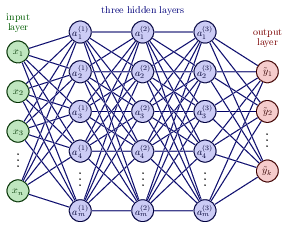
\includegraphics[width=0.5\linewidth]{latex//figures/nn1.png}
    \caption{\textbf{DNN}: Architecture of a deep neural network. An array of input data is sent via some weights and biases to a hidden layer $a_1$. Instead of sending the output of $a_1$ straight to an output layer, several more hidden layers are included.}
    \label{fig:dnn}
\end{figure}

%An example of a network with more layers is seen in Figure \ref{fig:dnn}, and while it looks a lot more complicated it is built of the same building blocks as the model seen in Figure \ref{fig:mlp}.

%A DNN (deep neural network) is a similar construction as the MLP, and in the literature the two often overlap, so it may be more helpful to just say what our two models were.\\Our input is the usual 28x28 dimensions of MNIST flattened to a 784 features long vector. 
%In the MLP this is sent to a single hidden layer of 500 features, and out output (which will be the latent space in the VAE) is set to 20 features.\\
%The DNN does the same, but it has an additional hidden layer after the first, consisting of 150 features.



% \subsection{RNN}
% Recurrent Neural Networks, or RNNs, are a type of neural network designed/structured to handle sequential, often time dependent, data. Where a typical Feed Forward Neural Network sends a single input vector \textbf{x} through an arbitrary number of hidden layers \textbf{h} to reach an output \textbf{y}, a recurrent network will send a separate input \textbf{x$<$t$>$} into a separate hidden layer \textbf{h$<$t$>$} for  every step of the sequence (or every time step), see \autoref{fig:RNN}. Each of these hidden layers will also receive input from the previous sequential hidden layer in order to incorporate the sequential nature of the input data. For each set of input data \textbf{x$<$t$>$} we will receive a separate output data \textbf{y$<$t$>$}, which in turn can be used to compute a loss for each sequential step. One will then require a total loss function over all steps, which can simply be the sum over all sequential steps. This loss is then backpropagated through the whole network. 

% \begin{figure}[!htb]
%  \centering
%  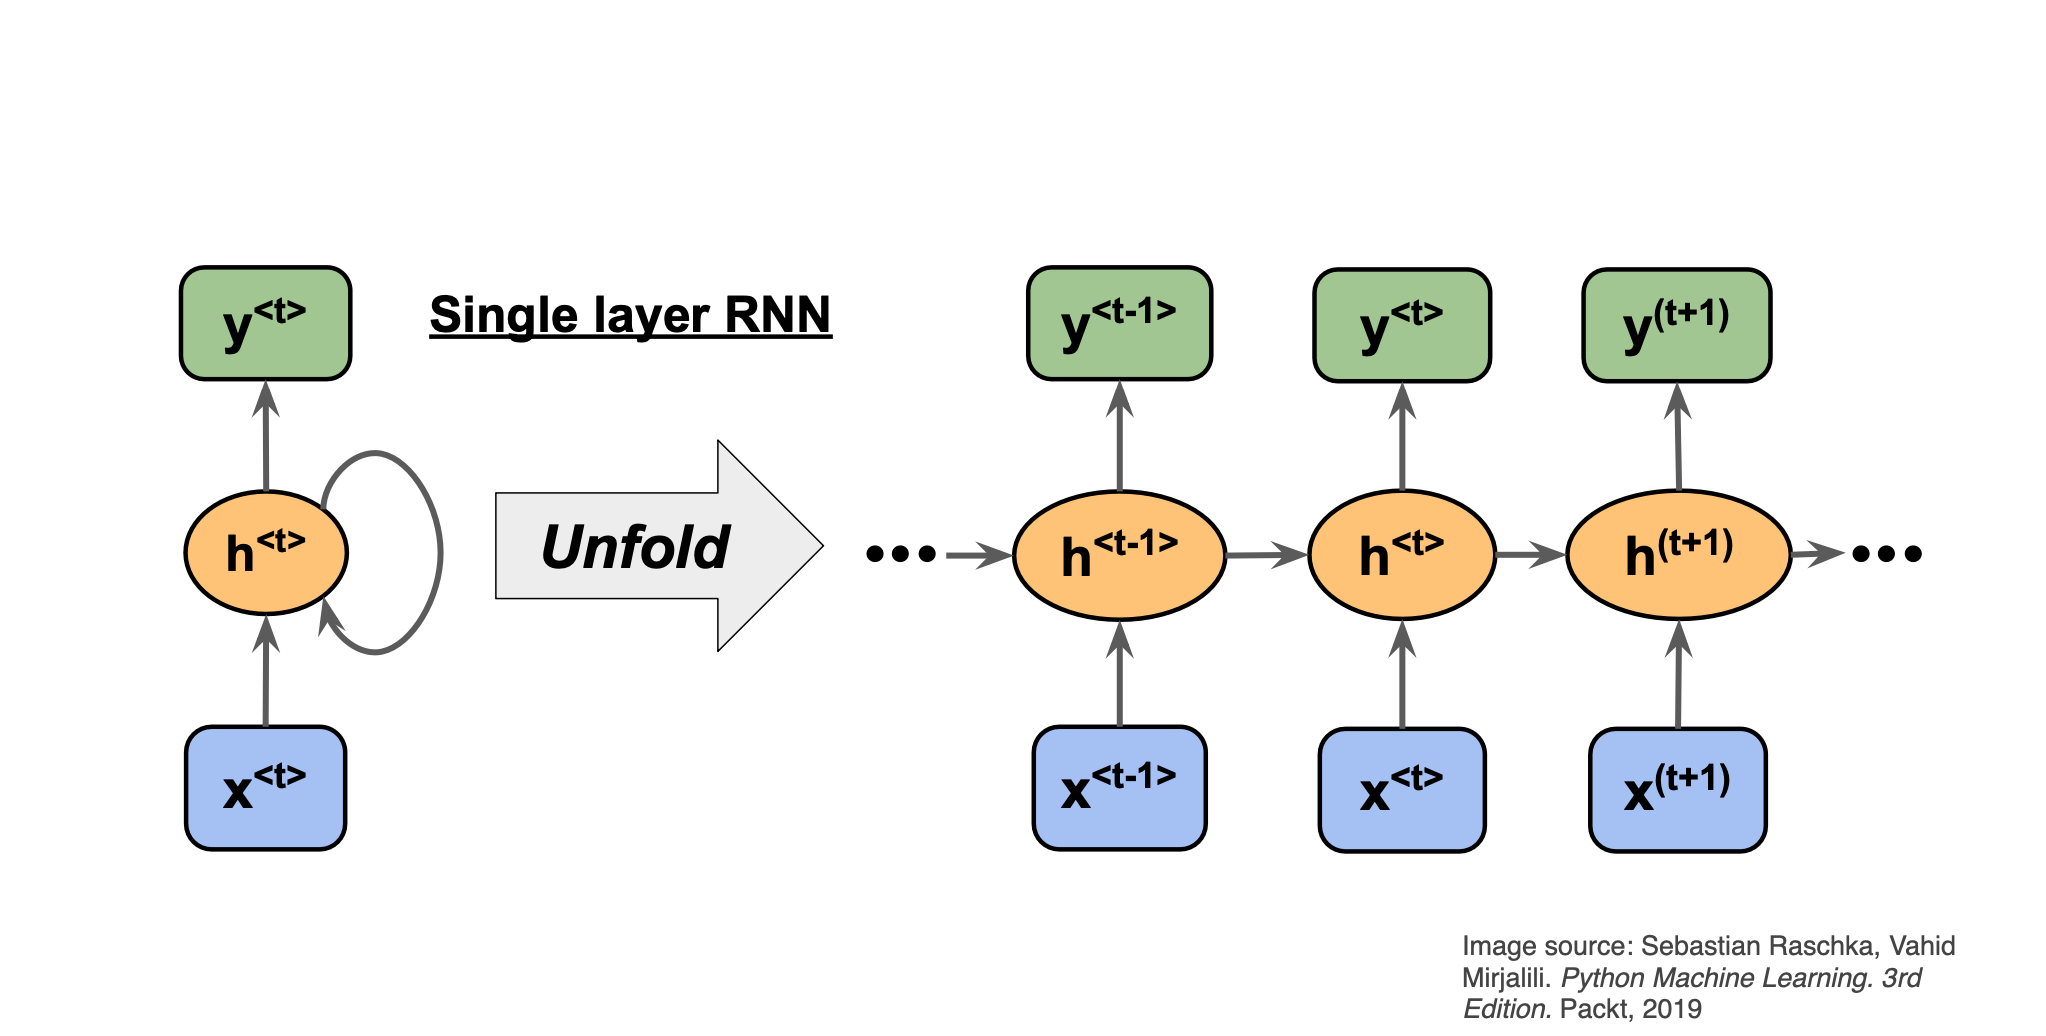
\includegraphics[scale=0.5]{RNN2.png}
%  % RNN2.png: 2046x1036 px, 144dpi, 36.09x18.27 cm, bb=0 0 1023 518
%  \caption{\textbf{Recurrent Neural Network architecture} Write here}
%  \label{fig:RNN}
% \end{figure}

% \subsubsection{The mathematics of RNNs}
% One can have other configurations of an RNN, such as not connecting hidden layers t and t-1, but rather the output of t-1 to the hidden layer of t, and other variants. But sticking with the architecture shown in \autoref{fig:RNN}, the relevant parameters can be seen in \autoref{fig:RNN_w}.

% \begin{figure}[!htb]
%  \centering
%  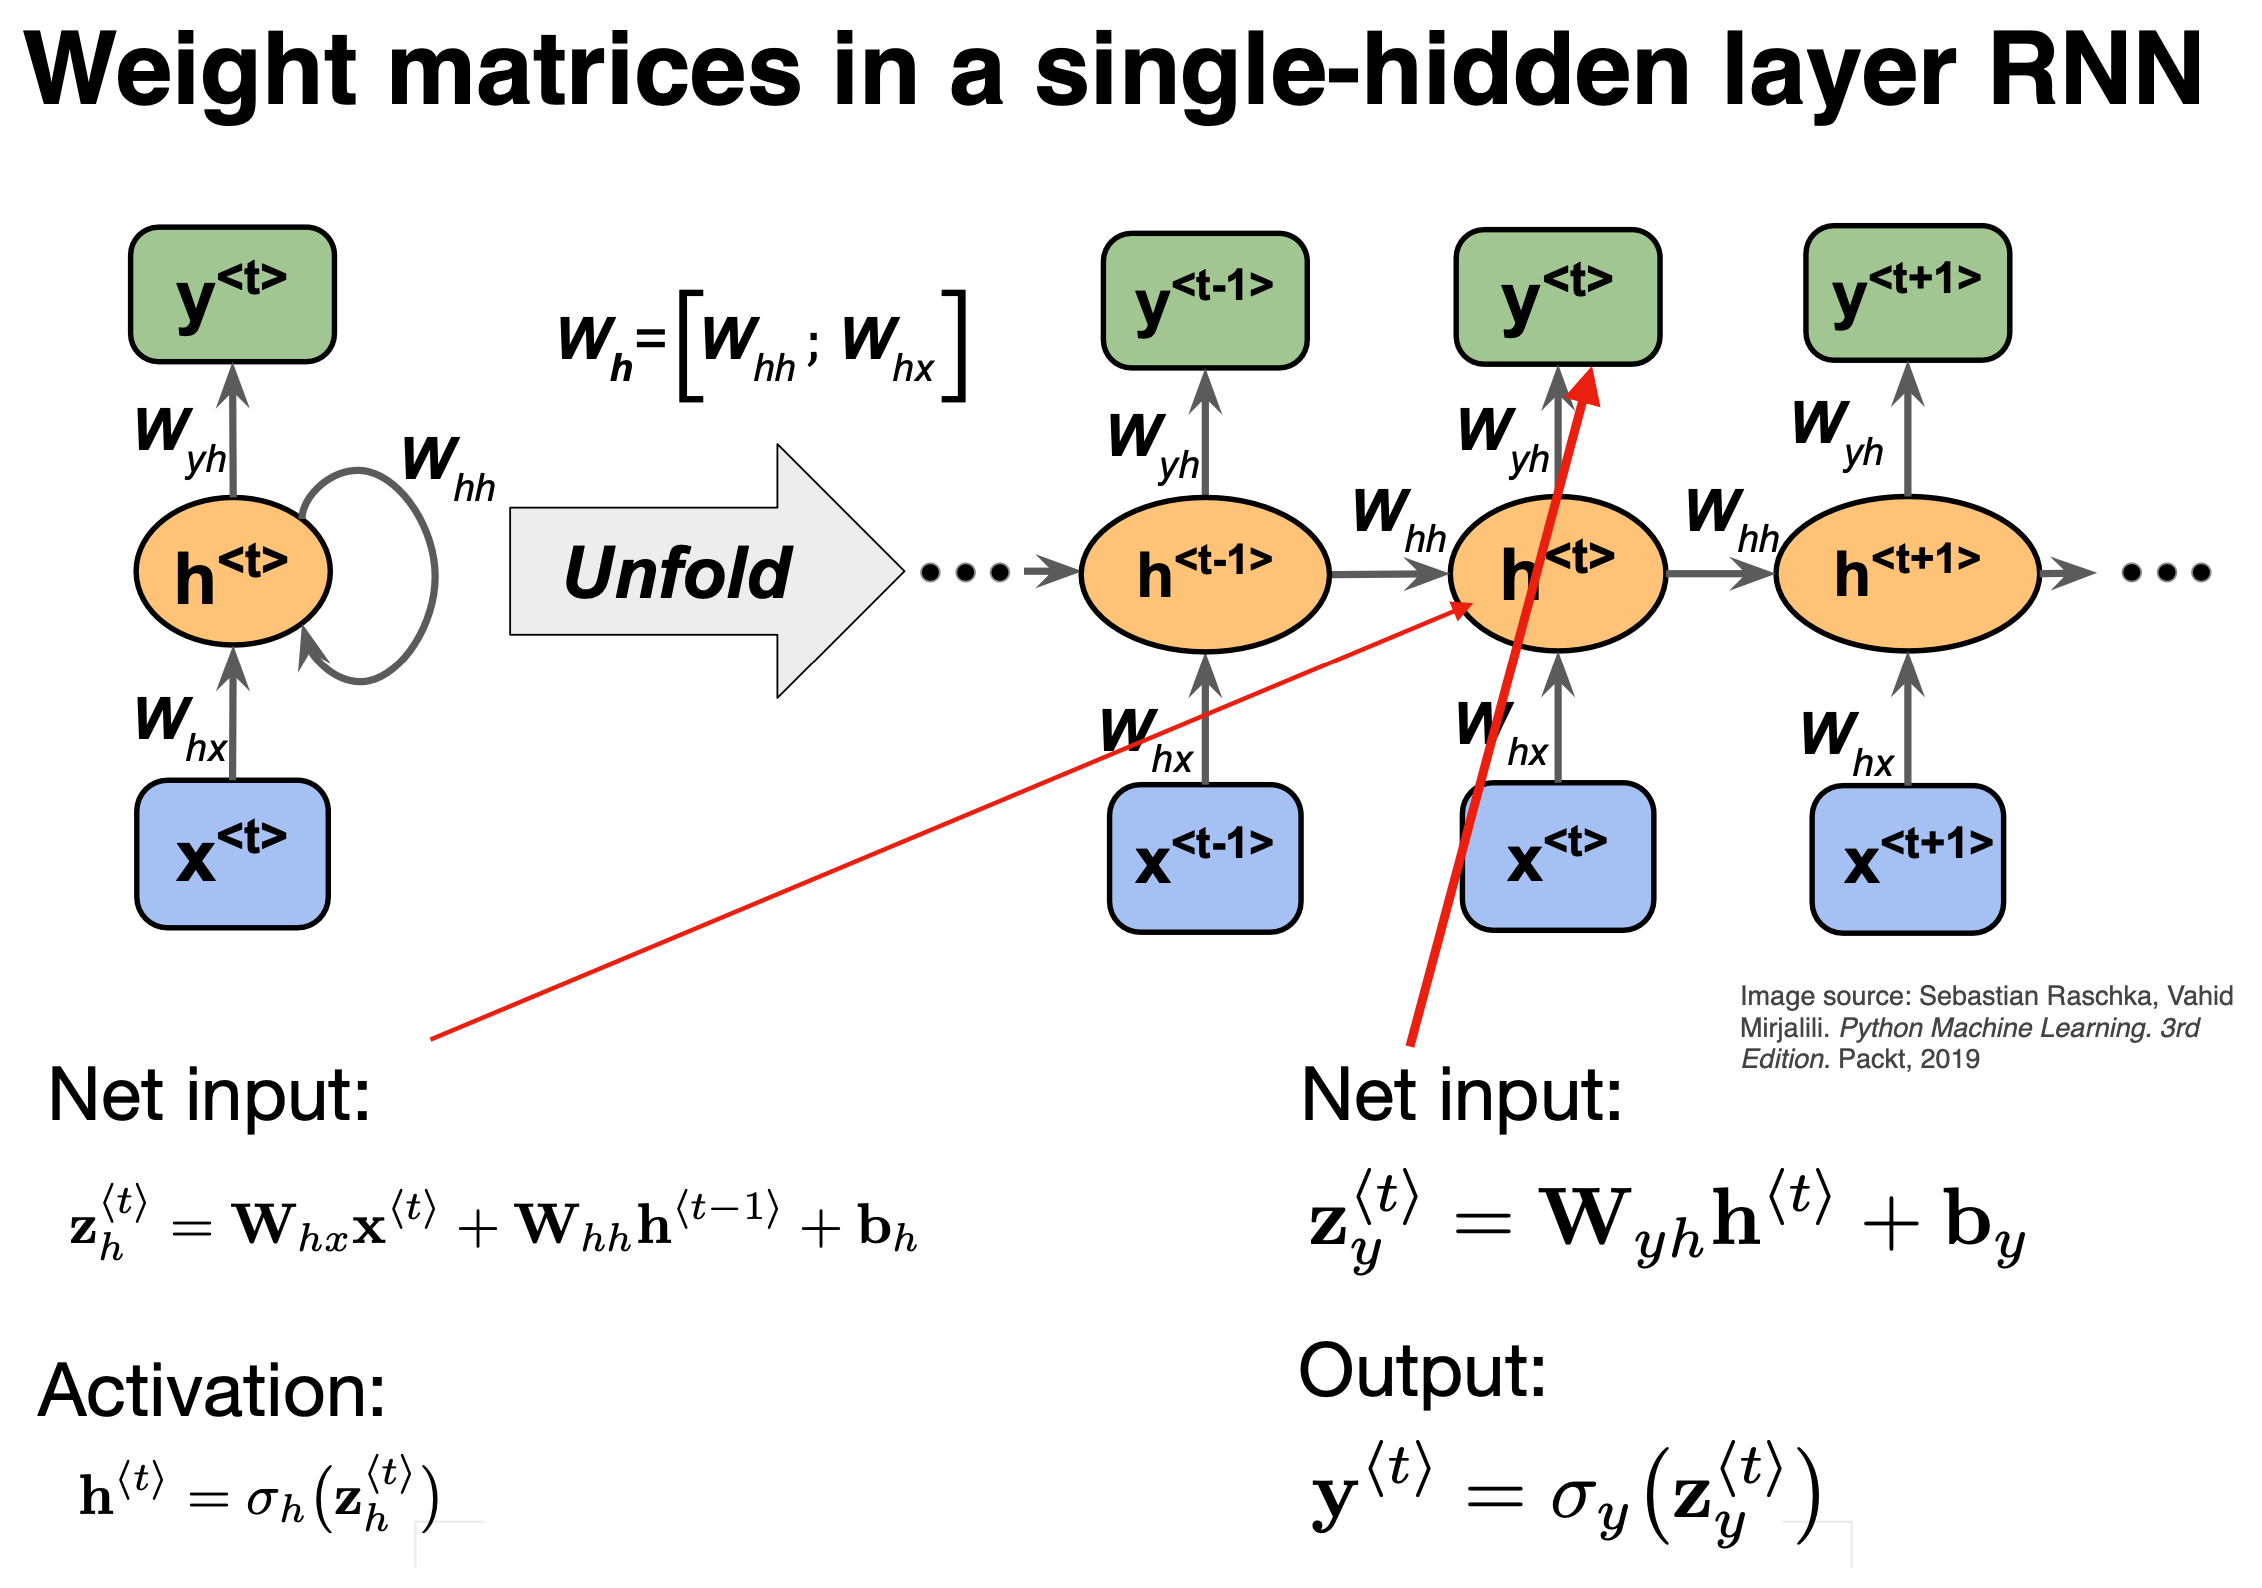
\includegraphics[trim={0cm 0cm 0cm 2.5cm},clip,scale=0.45]{RNN_w.png}
%  % RNN_w.png: 2262x1588 px, 144dpi, 39.90x28.01 cm, bb=0 0 1131 794
%  \caption{\textbf{RNN parameters}}
%  \label{fig:RNN_w}
% \end{figure}

% Here the inputs to each hidden layer depends on the previous hidden layer as well as the input for this time step, along with the inevitable bias. This input is sent into an activation function such as softmax, and then sent on to the output layer, as well as the next time step hidden layer.
% The total loss \textbf{L} can be computed as

% \begin{equation}
%  L = \sum_{t=1}^TL^{\langle t \rangle},
% \end{equation}

% where \textbf{L$^{\langle t \rangle}$} is the loss found at time step t. This loss is back propagated through the entire network, so now \textbf{h$^{<t-1>}$} receives 'input' from \textbf{h$^{<t>}$} as well as \textbf{y$^{<t-1>}$}.
% The back propagation is done sequentially by the chain rule; wrt to $W_{hh}$

% \begin{equation}
%  \frac{\partial L}{\partial W_{hh}} = \sum_{t=1}^T\frac{\partial L^{\langle t \rangle}}{\partial W_{hh}} = \sum_{t=1}^T \frac{\partial L^{\langle t \rangle}}{\partial y^{\langle t \rangle}}\frac{\partial y^{\langle t \rangle}}{\partial h^{\langle t \rangle}}\frac{\partial h^{\langle t \rangle}}{\partial W_{hh}}
% \end{equation}

% The final factor of this equation will depend on the weights $W_{hh}$ and the previous time step hidden layer (which again depends on the previous time step and so on.
% Thus we can write (note the lower case t in the summation, summin  only up to the current step):

% \begin{equation}
%  \frac{\partial h^{\langle t \rangle}}{\partial W_{hh}} = \sum_{k=1}^t \frac{\partial h^{\langle t \rangle}}{\partial h^{\langle k \rangle}} \frac{\partial h^{\langle k \rangle}}{\partial W_{hh}}
% \end{equation}

% The first factor here can be expanded

% \begin{equation}
%  \frac{\partial h^{\langle t \rangle}}{\partial h^{\langle k \rangle}} = \frac{\partial h^{\langle t \rangle}}{\partial h^{\langle t-1 \rangle}} \frac{\partial h^{\langle t-1 \rangle}}{\partial h^{\langle t-2 \rangle}}  \cdots \frac{\partial h^{\langle k+1 \rangle}}{\partial h^{\langle k \rangle}} = \prod_{i=k+1}^t \frac{\partial h^{\langle i \rangle}}{\partial h^{\langle i-1 \rangle}}
% \end{equation}

% If your data consists of many time steps this chain can become extremely long, both increasing computational costs and a long chain can cause exploding gradients as a small change in the initial conditions can lead to large changes in the outcome. 

% NICO:
% Section on handling exploding gradients? LSTM probably..
% Also, total loss should be divided by T (num timesteps) so scale of loss will not be sensitive to length of sequences. not relevant for our purposes I believe, w all sequences as long.

%----------------------------------------------------------------
\subsection{CNN}
%----------------------------------------------------------------

Convolutional Neural Networks (CNNs) are predominantly used in image processing tasks such as image recognition. They differ from other neural network types by incorporating convolution operations in one or more layers instead of typically used matrix multiplications. This architectural choice is tailored to leverage the typical spatial structure of images, characterized by dimensions of width, height, and depth, which helps optimize network performance compared to more general architectures. In CNNs, the 3D nature of input data (width, height, and channels) is preserved across hidden layers, which are specialized into specific types. The key of convolution lies in the application of kernels (typically N$x$N$x$F filters) across the input data. Each kernel slides over the input data with a predefined stride, computing outputs by performing a dot product operation within its receptive field. This process, illustrated in Figure \ref{fig:cnn}, transforms an initial 28x28x1 input image, for example, into a 28x28x32 output using a 5x5x32 kernel. In convolution operations like this, the focus is not on numerous weights and biases as in deep neural nets, but rather a smaller set of chosen parameters: 


\begin{itemize}
 \item \textbf{Kernel size}: The spatial dimensions of each filter, as well as the number of filters (N$x$N$x$F)
 \item \textbf{Stride}: The distance to move the kernel for each computation. The kernel is moved one stride length to the left each time until it reaches the end of the current row, then it will return to the initial position, move one stride down, and then repeat the whole process.
 \item \textbf{Padding}: Padding refers to adding a rim of zeros (typically) around your image, avoiding potential issues near the edges of the image, as well as to conserve the spatial dimension of the image being convolved.
\end{itemize}

\begin{figure}[H]
 \centering
 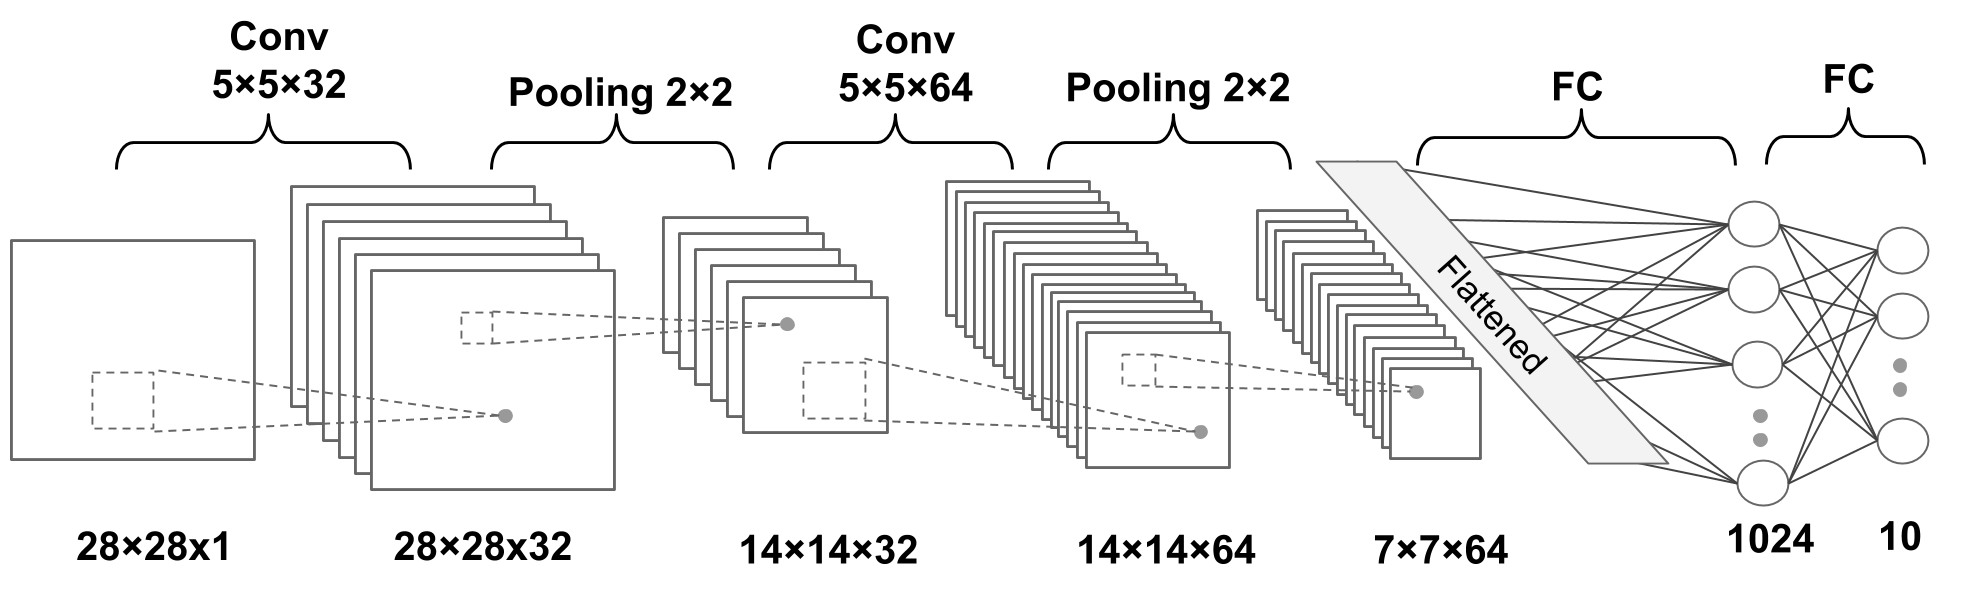
\includegraphics[scale=0.2]{deepcnn.png}
 % deepcnn.png: 1972x595 px, 72dpi, 69.57x20.99 cm, bb=0 0 1972 595
 \caption{\textbf{CNN architecture} A simple input of a grayscale image, of dimensions 28x28x1 is sent through two sets of convolutions and pooling before it is flattened, and sent through a set of fully connected layers (FC) in  the end.}
 \label{fig:cnn}
\end{figure}

Some benefits of such a network compared to a deep neural network are:
\begin{itemize}
 \item they take higher dimensional data as input
 \item not flattening input allows for learning local correlations in all dimensions. Good for feature extraction.
 \item instead of a heap of parameters to chose from, they are very limited per operation
 \item can do unsupervised classification and feature extraction/recognition
\end{itemize}

% %inside the window defined by the kernel, computing the output of local regions of the data.
%This step will typically increase the depth dimension size considerably, depending on the number of channels in the kernel used.\\

%Another important layer type in CNNs is the pooling layer, which decreases the spatial dimensions. In a way it is similar to what we did above, in that we create an N$x$N window again, whisch we apply in a similar manner all over the image. This time however, instead of doing a dot product over the image data and the kernel vaues, we simply find a way of representing the N$x$N data as one single data point. Two very popular methods are to either take the average over all values inside the window, or simply to pick the maximum value.
%In Figure \ref{fig:cnn} we see pooling being used in the second operation, where a 2x2 window is applied, quartering the spatial dimension of each channel. Note that this crude dimension reduction can loseinteresting features, so it is rarely chosen to be large.
%After a series of such convolutional and pooling layers, you will finally be prepared to do the classification, or whichever task you have for your network. The ouput of your final pooling layer is flattened into a single vector, and sent into one (ore more) fully connected (all to all) layer(s). The output of the final of these is used to perform your designated task.

Unlike deep neural networks that rely on extensive parameters, CNNs utilize a compact set of parameters per operation. Additionally, CNNs employ pooling layers to reduce spatial dimensions. Pooling involves applying an N$x$N window across the data and aggregating it into a single value, typically by taking the maximum or average. While effective for dimensionality reduction, pooling can discard nuanced features, thus smaller pool sizes are preferred. Following a sequence of convolutional and pooling layers, the final output is prepared for classification or another designated task. The output of the last pooling layer is flattened into a vector and fed into one or more fully connected layers, which perform the final computation.



\subsection{Visualizing the latent space}




Visualizing the latent space, where features are represented in a lower-dimensional form, helps when it comes to understanding data distributions and feature relationships. In order to do this, methods such as t-distributed stochastic neighbor embedding (t-SNE) are valuable for reducing high-dimensional data to a 2D or 3D embedding. t-SNE is a non-linear, unsupervised method that emphasizes proximity between data points in the latent space, revealing class distributions and similarities. To achieve this, t-SNE computes pairwise similarities between data points in the high-dimensional space using a Gaussian distribution, 

\begin{equation}
    p_{i|j}=\frac{\exp (-||x_i-x_j||^2/2\sigma_i^2)}{\sum_{k\neq i}\exp(-||x_i-x_k||^2/2\sigma_i^2)},
\end{equation}

with the probability that j is a neighbor if you are i. The probabilities will usually be symmetrized, $p_{ij}=(p_{j|i}+p_{i|j})/2N$, where N is the number of samples used. 

A similar probability distribution is created in the low dimensional visualization layer (or embedding space), using a Student t-distribution instead of the Gaussian distribution we used before: 

\begin{equation}
    q_{ij}=\frac{(1+||y_i-y_j||^2)^{-1}}{\sum_k\sum_{l\neq k}(1+||y_k-y_l||^2)^{-1}},
\end{equation}

where $q_{ii}=0$. We now have two probability distributions that we wish to make as similar as possible. This optimization process minimizes the Kullback-Leibler (KL) divergence between the high-dimensional and embedding space distributions, ensuring a faithful representation of data relationships in the reduced dimensionality.

%But this is something we have recently dealt with, and is done by minimizing the KL divergence!\\

If we call the embedding space distribution Q and the latent space distribution P, we have

\begin{equation}
    D_{KL}(P||Q)=\sum_{i\neq j}p_{ij}\log\frac{p_{ij}}{q_{ij}}
\end{equation}

as the expression we wish to minimize using gradient descent.
Running through these steps should result in a very low (2/3D) representation of a higher dimensional space, that can be used for visualizing classes.

By leveraging t-SNE, researchers can obtain insightful visualizations that facilitate the interpretation and analysis of complex data distributions, aiding tasks such as class separation and clustering in visual contexts. However, this computational method can be intensive for large datasets, requiring careful parameter tuning and computational resources to achieve optimal results.
